\documentclass{article}

% use Times
\usepackage{times}
% For figures
\usepackage{graphicx} % more modern
%\usepackage{subfigure} 
\usepackage{subcaption}


% For citations
\usepackage{natbib}

% For algorithms
\usepackage{algorithm}
\usepackage{algorithmic}

% As of 2011, we use the hyperref package to produce hyperlinks in the
% resulting PDF.  If this breaks your system, please commend out the
% following usepackage line and replace \usepackage{icml2016} with
% \usepackage[nohyperref]{icml2016} above.
\usepackage{hyperref}

% Packages hyperref and algorithmic misbehave sometimes.  We can fix
% this with the following command.
\newcommand{\theHalgorithm}{\arabic{algorithm}}

% Employ the following version of the ``usepackage'' statement for
% submitting the draft version of the paper for review.  This will set
% the note in the first column to ``Under review.  Do not distribute.''
\usepackage{icml2016} 
\usepackage{amsmath,amsfonts,amssymb}
\usepackage{dsfont}
\usepackage{booktabs}
\usepackage{relsize}
\usepackage{lmodern}
\usepackage{slantsc}
\usepackage{siunitx}
\sisetup{output-exponent-marker=\ensuremath{\mathrm{E}}}


\newcommand{\xsj}{\mathbf{\hat{x}}_j}
\newcommand{\xuj}{\mathbf{x}_j}
\newcommand{\xsi}{\mathbf{\hat{x}}_i}
\newcommand{\xui}{\mathbf{x}_i}
\newcommand{\ysi}{\hat{y}_i}
\newcommand{\ysj}{\hat{y}_j}
\newcommand{\yui}{y_i}
\newcommand{\sw}{s_{ \textsc{\relsize{-2}{\textsl{W}}} }}



% Employ this version of the ``usepackage'' statement after the paper has
% been accepted, when creating the final version.  This will set the
% note in the first column to ``Proceedings of the...''
%\usepackage[accepted]{icml2016}


% The \icmltitle you define below is probably too long as a header.
% Therefore, a short form for the running title is supplied here:
\icmltitlerunning{Transductive Unsupervised Domain Adaptation}

\begin{document} 

\twocolumn[
\icmltitle{Transductive Unsupervised Domain Adaptation}

% It is OKAY to include author information, even for blind
% submissions: the style file will automatically remove it for you
% unless you've provided the [accepted] option to the icml2016
% package.
\icmlauthor{Ozan Sener}{ozansener@cs.stanford.edu}
\icmladdress{Stanford University,
		     Stanford, CA 94304, USA}
		     \vspace{-2mm}
\icmladdress{Cornell University,
		     Ithaca, NY 14853, USA}
\icmlauthor{Hyun Oh Song}{hsong@cs.stanford.edu}
\icmladdress{Stanford University,
		     Stanford, CA 94304, USA}

\icmlauthor{Silvio Savarese}{ssilvio@stanford.edu}
\icmladdress{Stanford University,
		     Stanford, CA 94304, USA}
\icmlauthor{Ashutosh Saxena}{ashutosh@brainoft.com}
\icmladdress{Brain of Things,
		     Cupertino, CA 94304, USA}


% You may provide any keywords that you 
% find helpful for describing your paper; these are used to populate 
% the "keywords" metadata in the PDF but will not be shown in the document
\icmlkeywords{domain adaptation, transductive learning, metric learning, deep learning}

\vskip 0.3in
]

\begin{abstract} 
Recently, supervised learning with large scale labeled datasets and deep layered models has made a paradigm shift in diverse areas in learning and recognition. However, this approach still suffers generalization issues under the presence of a domain shift between the training and the test data distribution. In this regard, unsupervised domain adaptation algorithms have been proposed to directly address the domain shift problem. In this paper, we approach the problem from a transductive perspective. We incorporate the domain shift and the transductive target inference into our framework by jointly solving for an asymmetric similarity metric and the optimal transductive target label assignment. We also show that our model can easily be extended for deep feature learning in order to learn features which are discriminative in the target domain. Our experiments show that the proposed method significantly outperforms state-of-the-art algorithms in both object recognition and digit classification experiments by a large margin.
\end{abstract} 

\section{Introduction}
\label{intro}
Recently deep convolutional neural networks \cite{alexnet, vggnet, googlenet} have propelled unprecedented advances in artificial intelligence including object recognition, speech recognition, and image captioning. One of the major drawbacks of the method is that the network requires a lot of labelled training data to fit millions of parameters in the complex network model. However, creating such datasets with complete annotations is not only tedious and error prone but also extremely costly. In this regard, the research community have proposed different mechanisms such as semi-supervised learning \cite{semisup1,semisup2,semisup3}, transfer learning \cite{transfer1, transfer2}, weakly labelled learning, and domain adaptation. Of the approaches, domain adaptation is one of the most appealing techniques when a fully annotated dataset (i.e. ImageNet \cite{ImageNet}, Sports1M \cite{sports1m}) is available as a reference. 

Formally, the goal of unsupervised domain adaptation is: given a fully labeled source dataset and a unlabeled target dataset, learning a model which can generalize to the target domain while taking the domain shift across the datasets into account. The majority of the literature \cite{gong12, baochen15, fernando13, baochen16, tommasi13} in unsupervised domain adaptation formulates a learning problem where the task is to find a transformation matrix to align the labelled source data distribution to the unlabelled target data distribution. Although these approaches show promising results, it does not take the actual target inference procedure into the learning algorithm. We solve this problem by incorporating the unknown target labels into the training procedure.

Concretely, we formulate a unified framework where the domain transformation parameter and the target labels are jointly optimized in two alternating stages. In the transduction stage, given a fixed domain transform parameter, we jointly infer all target labels by solving a discrete multi-label energy minimization problem. In the adaptation stage, given a fixed target label assignment, we seek to find the optimal asymmetric metric  between the source and the target data. The advantage of the method is that the we can learn a domain transformation parameter which is aware of the subsequent transductive inference procedure. 

Following the standard evaluation protocol in the domain adaptation community, we evaluate our method on the digit classification task using MNIST \cite{mnist} and SVHN\cite{svhn} as well as the object recognition task using the Office \cite{office} dataset, and demonstrate state of the art performance in comparison to all existing unsupervised domain adaptation methods.  We will make our learned models as well as the source code available immediately upon acceptance.

\section{Related Work} 

This paper is closely related to two active research areas: (1) Unsupervised domain adaptation, and (2) Transductive learning.

\textbf{Unsupervised domain adaptation}: \cite{gong12, baochen15, fernando13, baochen16} proposed subspace alignment based approaches to unsupervised domain adaptation where the task is to learn a joint transformation and projection where the difference between the source and the target covariance is minimized. However, these methods learn the transform matrices on the whole source and target dataset without utilizing the the source labels. 

\cite{tommasi13} utilizes local max margin metric learning objective \cite{lmnn} to first assign the target labels with nearest neighbor scheme and then learn a distance metric to enforce that the negative pairwise distances are larger than the positive pairwise distances with a margin. However, this method learns a symmetric distance matrix shared by both the source and the target domains so the method is susceptible to the discrepancies between the source and the target distributions. Recently, \cite{ganin15, tzeng14} proposed a deep learning based method to learn domain invariant features via providing the reversed gradient signal from the binary domain classifiers. Although they perform better than aforementioned approaches, their accuracy is limited since domain invariance does not necessarily imply discriminative features in the target domain. 

\textbf{Transductive learning}: In the transductive learning literature \cite{transduction}, the model has access to unlabelled test samples during training. Recently, \cite{coclassification} tackled a classification problem where predictions are made jointly across all test examples in a transductive \cite{transduction} setting. The method essentially enforces the notion that the true labels vary smoothly with respect to the input data. In our work, we extend this notion to infer the multiclass labels of unsupervised target data in a k-NN graph. 

To summarize, our main contribution is to formulate joint optimization framework where we alternate between inferring target labels via discrete energy minimization (\textit{transduction}) and learning an asymmetric transformation (\textit{adaptation}) between source and target examples. Our experiments on digit classification using MNIST \cite{mnist} and SVHN\cite{svhn} as well as the object recognition experiments on Office \cite{office} datasets show state of the art results outperforming all existing methods by a substantial margin.


\section{Method} 
% !TEX root = domain_transduction.tex
\subsection{Problem Definition}
We are interested in the problem in which we have an unsupervised domain $\{\mathbf{x_i}\}_{i \in [N^u]}$ and a supervised domain $\{\mathbf{\hat{x}_i}, \hat{y}_i\}_{i \in [N^s]}$ such that $\mathbf{x_i}$ is the extracted feature for point $i$ and $y_i$ is the corresponding label. We also assume that unsupervised and supervised features have the same dimension i.e. $\mathbf{x}, \mathbf{\hat{x}} \in \mathcal{R}^d$

We consider an asymmetric similarity metric;
\begin{equation}
s(\mathbf{x_i}, \mathbf{\hat{x}_j}) = \mathbf{x_i}^\intercal \mathbf{W} \mathbf{\hat{x}_j}
\end{equation}
such that it is high if two points from supervised and unsupervised domains are similar to each other.

We approach to the problem from a transduction perspective; in other words, the main purpose of the method is recovering the labels $y_i$ for each unsupervised example $\mathbf{x_i}$. We consider the following objective function in order to compute $y_i$ as well as the similarity metric $\mathbf{W}$.

\begin{equation}
\begin{aligned}
\min_{\mathbf{W}, y_i} &\sum_{i \in [N^s]} &&[s(\mathbf{\hat{x_i}},\mathbf{x_{i^-}}) - s(\mathbf{\hat{x_i}},\mathbf{x_{i^+}}) + \alpha]_{+} \\
&s.t. \quad &&i^{+} = {\arg\max}_{j | y_j = \hat{y}_i} s(\mathbf{\hat{x_i}},\mathbf{x_{j}}) \\
&\quad &&i^{-} = {\arg\max}_{j | y_j \neq \hat{y}_i} s(\mathbf{\hat{x_i}},\mathbf{x_{j}}) 
\end{aligned}
\end{equation}

We solve this optimization problem via alternating minimization through iterating over solving for unsupervised labels $y_i$ and the similarity metric $\mathbf{W}$. We explain these two steps the following sections.

\subsection{Labeling Unsupervised Points}
We are using nearest neighbor rule in our labelling with an additional robustness metric. We first explain the nearest neighbor formulation then explain our extension. 

Given a similarity metric $\mathbf{W}$, the labeling with nearest neighbor rule is;
\begin{equation}
(y_i)^{pred} = \hat{y}_{{\arg\max}_j s(\mathbf{x_i}, \mathbf{\hat{x}_j})}
\end{equation}

Although the nearest neighbor rule is computationally inefficient, we solve the efficiency issues through usage of batches with stochastic gradient descent as well as an efficient implementation though OpenBLAS routines. We discuss these details in the implementation section of the paper.

Although the nearest neighbor rule is expected to work with a good metric, at the initial stage of the algorithm the metric will not be accurate enough. Hence, we need a robustness measure to handle the initial stage of the algorithm. Our robustness measure comes from the consistency of labels over the unsupervised data graph.

We create a k-NN graph over the unsupervised data points such that $\mathcal{N}(\mathbf{x_i})$ is the k  unsupervised data point nearest to $\mathbf{x_i}$ via the $l_2$ distance. After the k-NN graph is created, we solve the following optimization problem for labeling unsupervised data points;

\begin{equation}
\begin{aligned}
{\arg\min}_{y_i}  &\sum_{i \in N^u} \min_{\hat{y_j}=y_i} [1 - s(\mathbf{\hat{x_j}},\mathbf{x_{i}})] \\
&+ \lambda
\sum_{i \in N^u} \sum_{j \in \mathcal{N}(\mathbf{x_i})} [1 - \mathbf{x_i}^T \mathbf{x_j}] \mathds{1}(y_i \neq y_j)
\end{aligned}
\end{equation}

ADD NORMALIZATION STUFF TO MAKE THIS THING NON-NEGATIVE 


In its original form, this problem is multi-label energy minimization and it is submodular. However, solving this problem is still computationally inefficient. Therefore, we propose an approximate solution by minimizing the lower bound of this algorithm.
 \begin{equation}
 \begin{aligned}
 &\min_{\hat{y_j}=y_i} [1 - s(\mathbf{\hat{x_j}},\mathbf{x_{i}})] \\
  &\geq \left(\min_{ (y_j)^{pred} = y_i} [1 - s(\mathbf{\hat{x_j}},\mathbf{x_{i}})] \right) \mathds{1}[(y_j)^{pred} = y_i] \\ &+ \left(\min_{ (y_j)^{pred} \neq y_i} [1 - s(\mathbf{\hat{x_j}},\mathbf{x_{i}})] \right) \mathds{1}[(y_j)^{pred} \neq y_i]  
 \end{aligned}
 \end{equation}
 Moreover, the lower bound for the binary term can also be expressed as;
 {\small
 \begin{equation}
 \begin{aligned}
 &[1 - \mathbf{x_i}^T \mathbf{x_j}] \mathds{1}(y_i \neq y_j)   \\
 &\geq [1 - \mathbf{x_i}^T \mathbf{x_j}] \mathds{1}[y_i=(y_i)^{pred}, y_j=(y_j)^{pred}, (y_i)^{pred} \neq (y_j)^{pred}] \\
 &+  [1 - \mathbf{x_i}^T \mathbf{x_j}] \mathds{1}[y_i=(y_i)^{pred}, y_j \neq (y_j)^{pred}, (y_i)^{pred} = (y_j)^{pred}] \\
 \end{aligned}
 \end{equation}}
 
 In other words we convert the multi-label problem into binary problem with auxiliary variables \mbox{$y^b_i = \mathds{1}[y_i = (y_i)^{pred}]$} and the binary energy minimization problem becomes;
 
 \begin{equation}
 \begin{aligned}
&{\arg\min}_{y^b_i}  \sum_{i \in N^u} E_i(y^b_i) + \sum_{i \in N^u} \sum_{j \in \mathcal{N}(\mathbf{x_i})} E_{i,j} (y^b_i, y^b_j) \\
&E_i(y^b_i) = \left\{ \begin{array}{cc} \min_{ (y_j)^{pred} = y_i} [1 - s(\mathbf{\hat{x_j}},\mathbf{x_{i}})] & y^b_i = 1
\\  \min_{ (y_j)^{pred} \neq y_i} [1 - s(\mathbf{\hat{x_j}},\mathbf{x_{i}})] & y^b_i = 0 \\
 \end{array} \right. \\
&E_{i,j}(y^b_i,y^b_j) = \left\{ \begin{array}{cc} 1 - \mathbf{x_i}^T \mathbf{x_j}  & (y_i)^{pred}=(y_i)^{pred}, y^b_i \neq y^b_j \\ 1 - \mathbf{x_i}^T \mathbf{x_j} & (y_i)^{pred} \neq (y_i)^{pred}, y^b_i = y^b_j \\ 
0 & o.w. \\ \end{array} \right. \\
\end{aligned}
 \end{equation}
Although this function is not sub-modular, it can still be very efficiently minimized via QPBO(quadratic pseudo boolean optimization)\cite{kolmogrov} internally using min-cut/max-flow. After the energy minimization, the unsupervised data points with label $y_i=1$ keep their NN labels. For the rest, we sort them by using $\max_{j \in \mathcal{N}(\mathbf{x_i})} \mathbf{x_i}^T \mathbf{x_j}$ and start from the maximum similarity one and greedily assign labels as;
\begin{equation}
y_i = {\arg\max}_{y_i}  \max_{\hat{y_j}=y_i}  s(\mathbf{\hat{x_j}},\mathbf{x_{i}})]+ \lambda  \sum_{j \in \mathcal{N}(\mathbf{x_i})\cap P}  \mathbf{x_i}^T \mathbf{x_j} \mathds{1}(y_i \neq y_j)
\end{equation}
where $P$ is the set of points with label $y^b_i=1$ and the points which are already processed via the greedy operation. We  continue until all other points having the binary label $y^b_i=0$ is labeled.

\subsection{Learning Similarity Metric}
Given the predicted labels $y_i$ for unsupervised data points $\mathbf{x_i}$, we learn the asymmetric metric following the LMNN(Large Margin Nearest Neighbour)\cite{lmnn} construction. We start with finding the nearest positive and negative examples through;
\begin{equation}
\begin{aligned}
&i^{+} = {\arg\max}_{j | y_j = \hat{y}_i} s(\mathbf{\hat{x_i}},\mathbf{x_{j}}) \\
&i^{-} = {\arg\max}_{j | y_j \neq \hat{y}_i} s(\mathbf{\hat{x_i}},\mathbf{x_{j}}) 
\end{aligned}
\end{equation}
Then, we construct the loss function with regularizer;
\begin{equation}
\min_{\mathbf{W}, y_i} \sum_{i \in [N^s]} [s(\mathbf{\hat{x_i}},\mathbf{x_{i^-}}) - s(\mathbf{\hat{x_i}},\mathbf{x_{i^+}}) + \alpha]_{+} + r(\mathbf{W})
\end{equation}
which is convex in terms of the similarity metric $\mathbf{W}$ if the regularizer is convex; and we optimize it by using Stochastic gradient descent through the subgradient $\frac{\partial loss (y_i, \mathbf{W})}{\partial \mathbf{W}} =$
\begin{equation}
\sum_{i \in [N^s]} \mathds{1}[s(\mathbf{\hat{x_i}},\mathbf{x_{i^-}}) - s(\mathbf{\hat{x_i}},\mathbf{x_{i^+}}) > \alpha] \left( \mathbf{\hat{x_i}}\mathbf{x_{i^-}}^\intercal - \mathbf{\hat{x_i}}\mathbf{x_{i^+}}^\intercal  \right)  + \frac{\partial r ( \mathbf{W})}{\partial \mathbf{W}}
\end{equation}
As a regularizer we are using the Frobenius norm of the similarity matrix as $r(\mathbf{W})=\frac{1}{2}\|\mathbf{W}\|_F^2$ 

\subsection{Learning Features}
\subsection{Learning with Synthetic Data}



\section{Experimental Results}
% !TEX root = domain_transduction.tex
We evaluate our algorithm on various unsupervised domain adaptation tasks while focusing on two different problems, hand-written digit classification and object recognition. For each experiment, we use three domains and evaluate all adaptation scenarios.

\begin{table*}[ht]
\setlength{\tabcolsep}{3pt}
\vspace{-3mm}
\caption{Accuracy of our method and the state-of-the-art algorithms on Office dataset and various adaptation settings}
\label{tab:res}
\begin{sc}
\begin{center}
\begin{small}
\resizebox{\columnwidth}{!}{%
\begin{tabular}{@{}rcccccc@{}} \toprule 
 Source & Amazon & D-SLR & Webcam & Webcam &Amazon & D-SLR \\
 Target & Webcam & Webcam & D-SLR & Amazon & D-SLR & Amazon \\
 \midrule
GFK \cite{gong2012} & $.398$ & $.791$ & $.746 $ & $.371$ & $.379$ & .379   \\
SA* \cite{fernando13} & $.450$ & $.648$ & $.699$ & $.393$ & $.388$ & $.420$ \\
DLID \cite{chopra13} & $.519$ & $.782$ & $.899$ & -&- &- \\
DDC \cite{tzeng14} & $.618$ & $.950$ & $.985$ & $.522$ & $.644$& $.521$\\
DAN \cite{wang15} & $.685$ & $.960$ & $.990$ & $.531$ & $.670$ & $.540$ \\
Backprop \cite{ganin15} & $.730$ &$.964$ & $.992$ & $.536$ & $.728$ & $.544$\\
\midrule
Source Only & $.642$ & $.961$ & $.978$ & $.452$ & $.668$ & $.476$ \\
Our Method (no reject/no prop) & $.727$ &.952 & $.915$ & $.575$ & $.791$ & $.521$ \\
Our Method (no reject) & $.804$ &$.962$ & $.989$ & $.625$ & $.839$ & $.567$ \\
Our Method (full) & $\mathbf{.814}$ & $\mathbf{.971}$ & $\mathbf{.993}$ & $\mathbf{.663}$ & $\mathbf{.847}$ & $\mathbf{.601}$ \\
\bottomrule
\end{tabular}}
\end{small}
\end{center}
\end{sc}
\vspace{-5mm}
\end{table*}

\subsection{Dataset}
We use MNIST~\cite{mnist}, Street View House Number~\cite{svhn} and the artificially generated version of MNIST -MNIST-M-~\cite{ganin15} to experiment our algorithm on the digit classification task. MNIST-M is simply a blend of the digit images of the original MNIST dataset and the color images of BSDS500~\cite{bsds500} following the method explained in \cite{ganin15}. Since the dataset is not distributed directly by the authors, we generated the dataset using the same procedure and further confirmed that the performance is the same as the one reported in \cite{ganin15}. Street View House Numbers dataset is a collection of house numbers collected directly from Google street view images. Each of these three domains are quite different from each other and among many important differences, the most significant ones are MNIST being grayscale and the others being colored, and SVHN images having extra confusing digits around the centered digit of interest. Moreover, all three domains are large-scale having at least 60k examples over 10 classes. 

\begin{wraptable}{r}{0.5\textwidth}
%\begin{table}[ht]
\setlength{\tabcolsep}{3pt}
\caption{Accuracy on the digit classification task.}
\label{tab:res2}
\begin{sc}
\begin{small}
\resizebox{0.5\textwidth}{!}{%
\begin{tabular}{@{}r@{\hskip 1mm}c@{\hskip 1mm}c@{\hskip 1mm}c@{\hskip 1mm}c@{}} \toprule 
Source & M-M & MNIST  & SVHN & MNIST \\
Target&  MNIST & M-M & MNIST & SVHN\\
 \midrule
SA* \cite{fernando13}& $.523$ & $.569$ & $.593$ & $.211$ \\
BP \cite{ganin15} &$.732$ & $.766$ & $.738$ & $.289$ \\
\midrule
Source Only  & $.483$ & $.522$  &.549 & $.162$  \\
Our Method & $\mathbf{.835}$ & $\mathbf{.855}$ & $\mathbf{.774}$ & $\mathbf{.323}$\\
 \bottomrule
\end{tabular}}
\end{small}
\end{sc}
\end{wraptable}

In addition, we use the Office~\cite{office} dataset to evaluate our algorithm on the object recognition task. Office dataset includes images of the objects taken from Amazon, captured with a webcam and captured with a D-SLR. Differences between domains include the white background of Amazon images vs realistic webcam images, and the resolution differences. The Office dataset has fewer images, with a maximum of 2478 per domain over 31 classes. %On the other hand, it has larger number of classes over 31 categories.

\subsection{Baselines}
We compare our method with a variety of methods with and without feature learning. Considering the two different lines of work, \textbf{SA*}\cite{fernando13} is the dominant state-of-the-art approach not employing any feature learning, and \textbf{Backprop(BP)}\cite{ganin15} is the dominant state-of-the-art employing feature learning. We use the available source code of \cite{ganin15} and \cite{fernando13} and following the evaluation procedure in \cite{ganin15}, we choose the hyper-parameter of \cite{fernando13} as the highest performing one among various alternatives. We also compare our method with the \textbf{source only} baseline which is a convolutional neural network trained only using the source data. This classifier is clearly different from our nearest neighbor classifier; however, we experimentally validated that CNN always outperformed the nearest neighbor based classifier. Hence, we report the highest performing source only method.

\subsection{Implementation Details}
\label{imp_det}
Although our algorithm has very few hyper-parameters and we choose most of them either using cross-validation or exhaustive grid search, our algorithm uses an existing differentiable feature function. Following the unparalleled success of convolutional neural networks (CNNs), we use CNNs as our feature functions.  We consider the last fully connected layer as domain specific feature ($\theta_s$, $\theta_t$) and the rest as common network $\theta_c$. Common network weights are tied between domains. In order to have a fair comparison with existing algorithms, we follow the same architecture used by \cite{ganin15} by only changing the final feature dimensionality (embedding size). We use the following architectures for domains:

\noindent \textbf{MNIST} and \textbf{SVHN:} LeNet\cite{lenet} as; \includegraphics[width=0.5\columnwidth]{lenet}

\noindent \textbf{Office:} AlexNet\cite{alexnet} as; 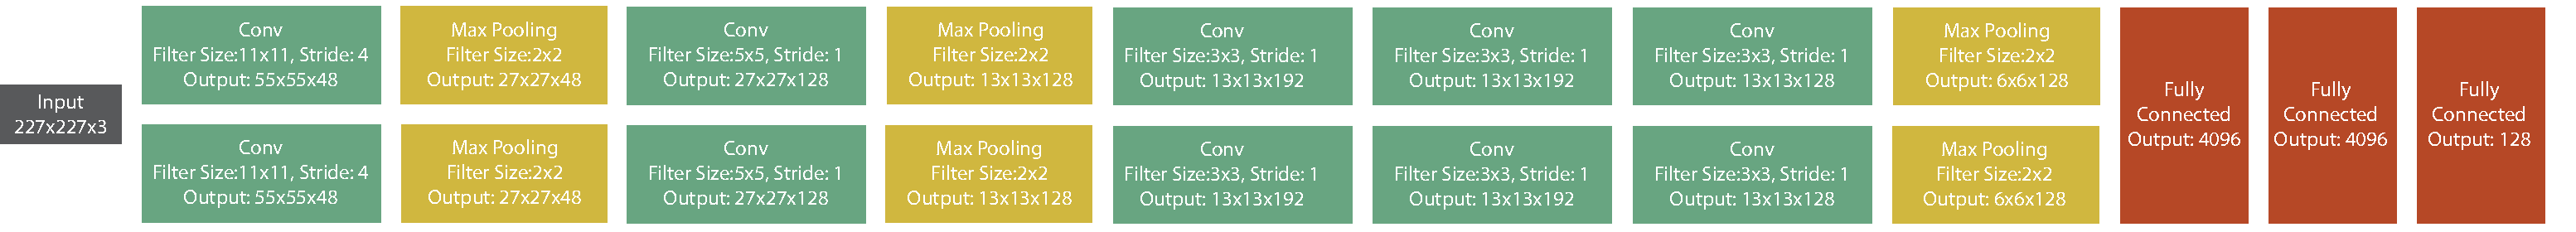
\includegraphics[width=0.55\columnwidth]{alexnet}

where \textbf{C} is convolution, \textbf{P} is max-pooling, \textbf{R} is ReLU and \textbf{F} is fully connected layer. 

Since the office dataset is quite small, we do not learn the full network for office experiments and instead we only optimize for fully connected layers initializing with the weights pre-trained on ImageNet. In all of our experiments, we set the feature dimension as $128$. We use stochastic gradient descent to learn the feature function with AdaGrad\cite{adagrad}. We initialize variables with truncated normals having unit variance and use the learning rate \SI{2.5e-4}  and the batch size $256$. We start the rejection penalty with $\gamma=0.5$ and linearly increases with each epoch as $\gamma=\frac{epoch\quad cnt}{20}$.

\subsection{Evaluation Procedure}
We evaluate all algorithms in fully transductive setup following the standard evaluation setup of \cite{office}.  We feed training images and labels of the first domain as the source and training images of the second domain as the target. We further evaluate the accuracy on the target domain labels as the ratio of correctly labeled images to all target images.

\subsection{Results}
Following the fully transductive evaluation, we summarize the results in Table~\ref{tab:res} and Table~\ref{tab:res2}. Table~\ref{tab:res} summarizes the results on the object recognition task using office dataset whereas  Table~\ref{tab:res2} summarizes the digit classification task on MNIST and SVHN.

Table~\ref{tab:res}\&\ref{tab:res2} shows results on object recognition and digit classification tasks exhaustively covering all adaptation scenarios. Our algorithm shows state-of-the-art performance. Moreover, our algorithm significantly outperforms all state-of-the-art methods when there is a large domain difference such as MNIST$\leftrightarrow$MNIST-M, MNIST$\leftrightarrow$SVHN, Amazon$\leftrightarrow$Webcam and Amazon$\leftrightarrow$D-SLR. Our hypothesis is that the state-of-the-art algorithms like \cite{ganin15} are seeking for set of features invariant to the domains whereas we seek for an explicit similarity metric explaining both differences and similarities of domains. In other words, instead of seeking for an invariance, we seek for an equivariance.

\iffalse
\begin{wrapfigure}{r}{0.5\textwidth}
\vspace{-1mm}
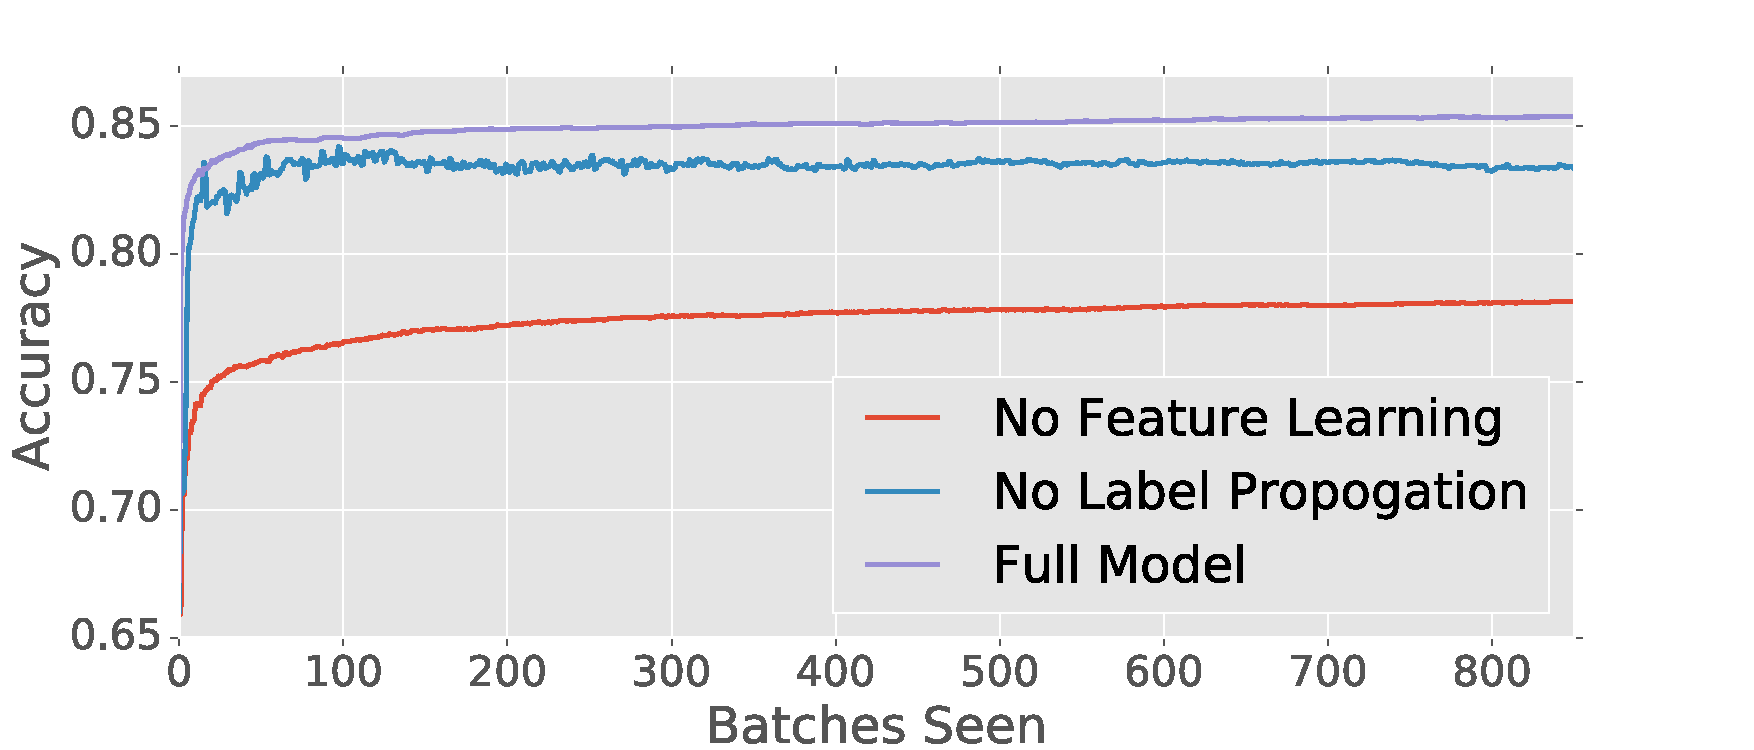
\includegraphics[width=0.5\textwidth]{no_feature_propogation}
\vspace{-6mm}
\caption{Accuracy vs number of iterations for our method and its variant without label propagation as well as the variant without feature learning. As the figure suggests the label propagation increases both the stability of the gradients as well as the final accuracy. Moreover, the feature learning also has a significant effect on the accuracy.}
\label{fllprop}
\end{wrapfigure}
\fi

Table~\ref{tab:res2} further suggests our algorithm is the only one which can generalize that well from MNIST to SVHN dataset. Clearly the features which are learned from MNIST cannot generalize to SVHN since the SVHN has concepts like color and occlusion which are not available in MNIST. Hence, our algorithm learns SVHN specific features by enforcing accurate transduction in the adaptation stage.

Another interesting conclusion is the asymmetric nature of the results. For example, the accuracy of adapting webcam to amazon and adapting Amazon to webcam is significantly different in Table~\ref{tab:res}. The similar behavior exists in MNIST and SVHN domains as well in Table~\ref{tab:res}. This observation validates the importance of an asymmetric modeling.

\subsubsection{Qualitative Analysis}
To further study the learned representations as well as the similarity metric, we perform a series of qualitative analysis in the form of nearest neighbor analyses and tSNE\cite{tsne} plots.

Figure~\ref{fig:nn} visualizes example target images from MNIST and their corresponding source images. First of all, both our experimental procedure and qualitative analysis suggest that MNIST and SVHN are the two domains with the largest difference. Hence, we believe MNIST$\leftrightarrow$SVHN is very challenging set-up and despite the huge visual differences, our algorithm results in accurate nearest neighbors.

Figure~\ref{fig:nnoffice} visualizes the example target images from webcam and their corresponding nearest source images from Amazon. The difference between invariance and equivariance is more clear in the tSNE plots of the Office dataset in Figure~\ref{fig:tsne} as well as digit classification task Figure~\ref{fig:tsnedigit}. In Figure~\ref{fig:tsne}, we plot the distribution of features before and after adaptation for source and target while color coding class labels. As Figure~\ref{fig:tsne} suggests, the source domain is well clustered according to the object classes with and without adaptation. Moreover, this is expected since the features are specifically fine-tuned to the source domain before the adaptation starts. However, target domain features have no structure before adaptation. This is also expected since the algorithm did not see any image from the target domain. After the adaptation, target images also get clustered according to the object classes. 

\begin{wrapfigure}{r}{0.4\textwidth}
\begin{small}
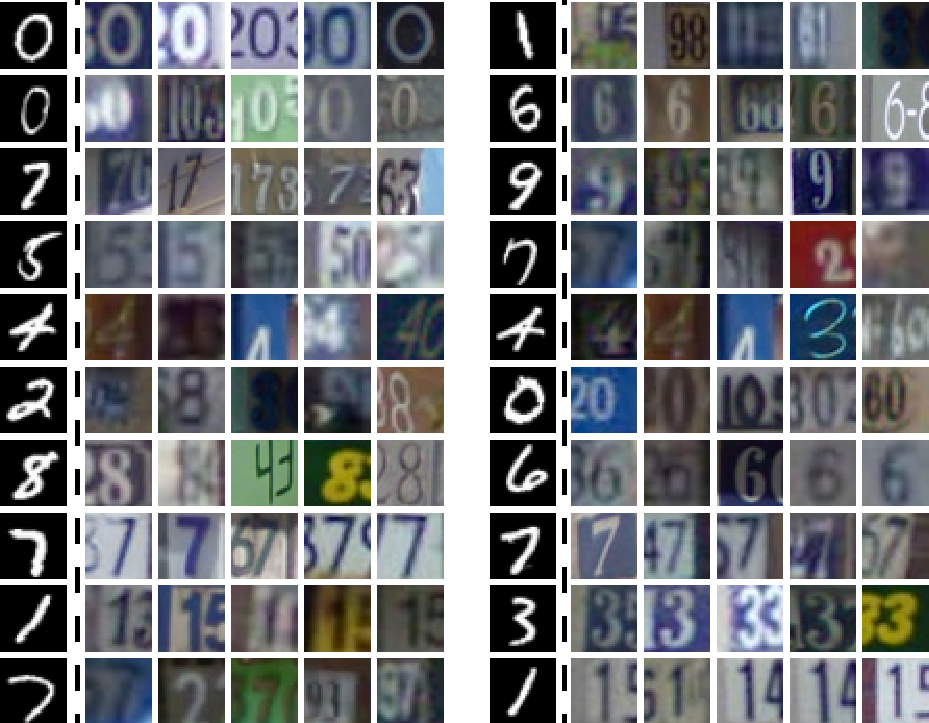
\includegraphics[width=0.4\textwidth]{nndig}
\vspace{-5mm}
\caption{Example nearest neighbors for SVHN$\rightarrow$MNIST experiment. We show an example MNIST image and 5-NN SVHN images. Please note the large domain difference.}
\label{fig:nn}
%\end{figure}
%\begin{figure}[ht]
\includegraphics[width=0.4\textwidth]{nnfi-01.png}
\caption{Example nearest neighbors for Amazon$\leftrightarrow$Webcam experiment. We show an example source image and 3-NN target images. }
%The drop in the accuracy after the nearest neighbors is expected since our loss function only models the nearest one.}
\label{fig:nnoffice}
\end{small}
\vspace{-1cm}
\end{wrapfigure}


In Figure~\ref{fig:tsnedigit}, we show the digit images of source and target after the adaptation. Clearly, the target is well clustered according to the classes and source is not very well clustered although it has some structure. Since we learn the entire network for digit classification, our networks learn discriminative features in the target domain as our loss depends directly on classification scores in target domain. Moreover, discriminative features in target arises because of the transductive modeling. In comparison, state of the art domain invariance based algorithms only try to be invariant to the domains without explicit modeling of discriminativeness on the target domain. Hence, our similarity metric explicitly models the relationship between the domains and results in an equivariant model while enforcing discriminative behavior in the target. We also draw lines between the nearest neighbor images of source and target images to show the accuracy of the metric function. Moreover, the nearest neighbors are quite accurate confirming the quantitative results. 

\subsubsection{Label propagation \& reject option}
In order to evaluate the effect of having a robust label propagation and reject option, we compare our method with self baselines. We compare our algorithm with the version neither include label propagation nor include the reject option as well as a version only include propagation. We denote them with no reject/no prop and no reject respectively. We tabulate the accuracy results from Office dataset in Table~\ref{tab:res}. Results suggests that both feature learning and reject option are crucial for successful transduction. 
%Another interesting observation is the unstable behavior when we disable label propagation. This is also expected since without label propagation, the labeling stage will have more mis-classifications and they will decrease the accuracy of the metric.
%>>>>>>> 495209cbd03d496cea6aa34df03ce5686deb5946


  
\begin{figure*}[ht]
    \begin{subfigure}[b]{0.25\textwidth}
        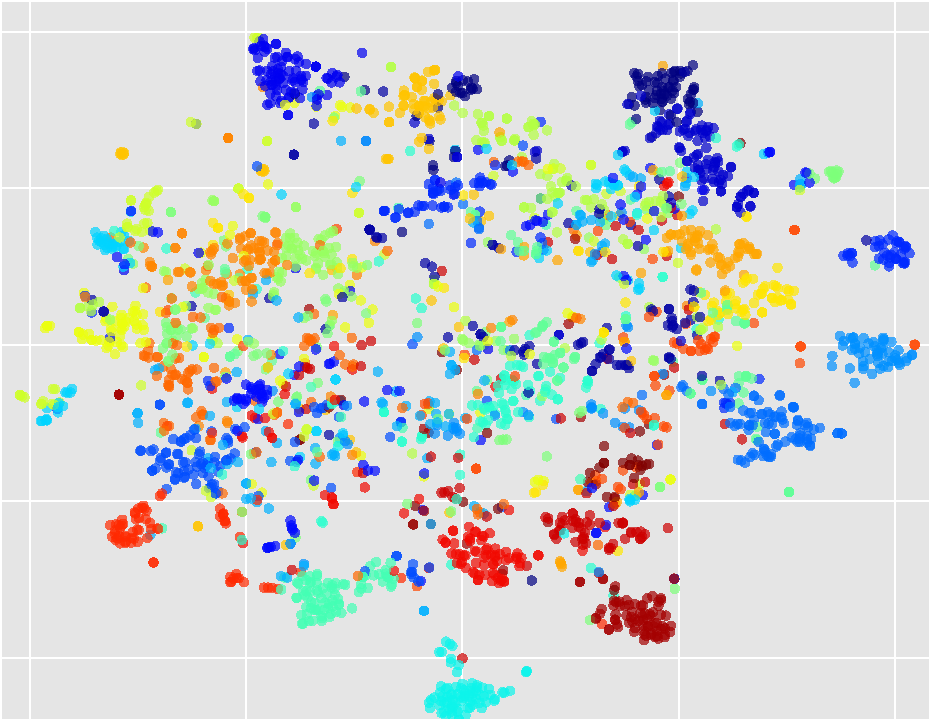
\includegraphics[width=\textwidth]{before_c_s_c}
        \caption{S. w/o Adaptation}
        \label{fig:gull}
    \end{subfigure}~\begin{subfigure}[b]{0.25\textwidth}
        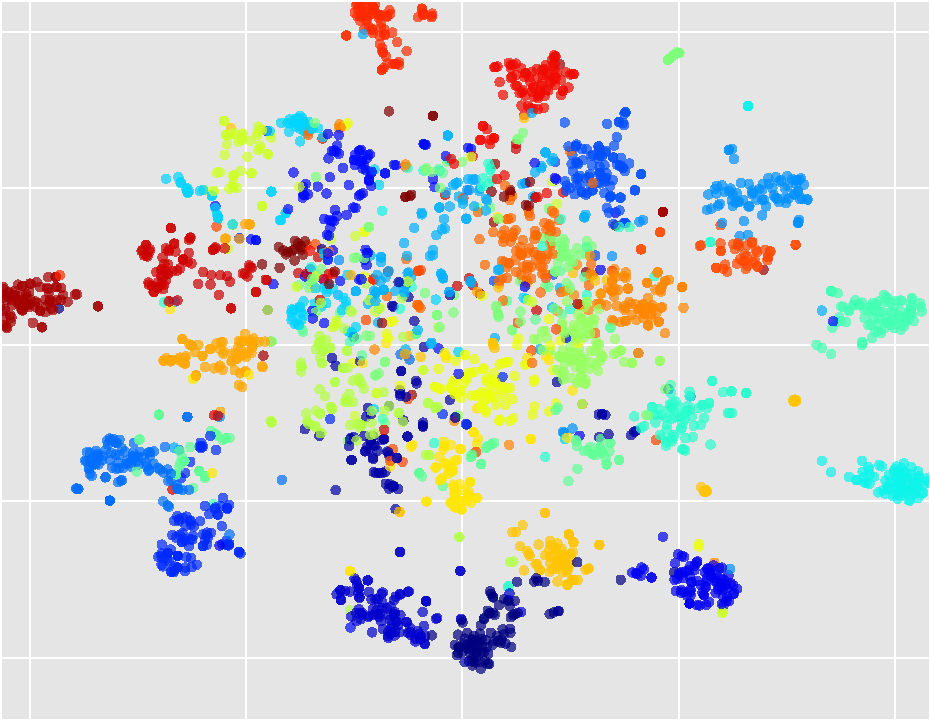
\includegraphics[width=\textwidth]{after_c_s_c}
        \caption{S. with Adaptation}
    \end{subfigure}~\begin{subfigure}[b]{0.25\textwidth}
        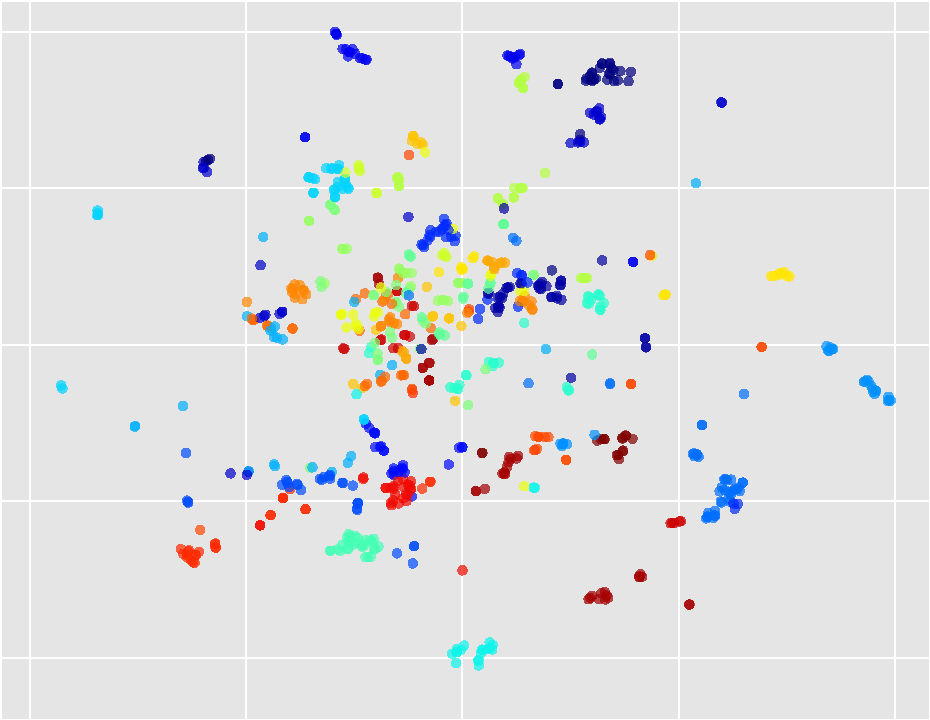
\includegraphics[width=\textwidth]{before_c_t_c}
        \caption{T w/o Adaptation}
        \label{fig:gull}
    \end{subfigure}~\begin{subfigure}[b]{0.25\textwidth}
        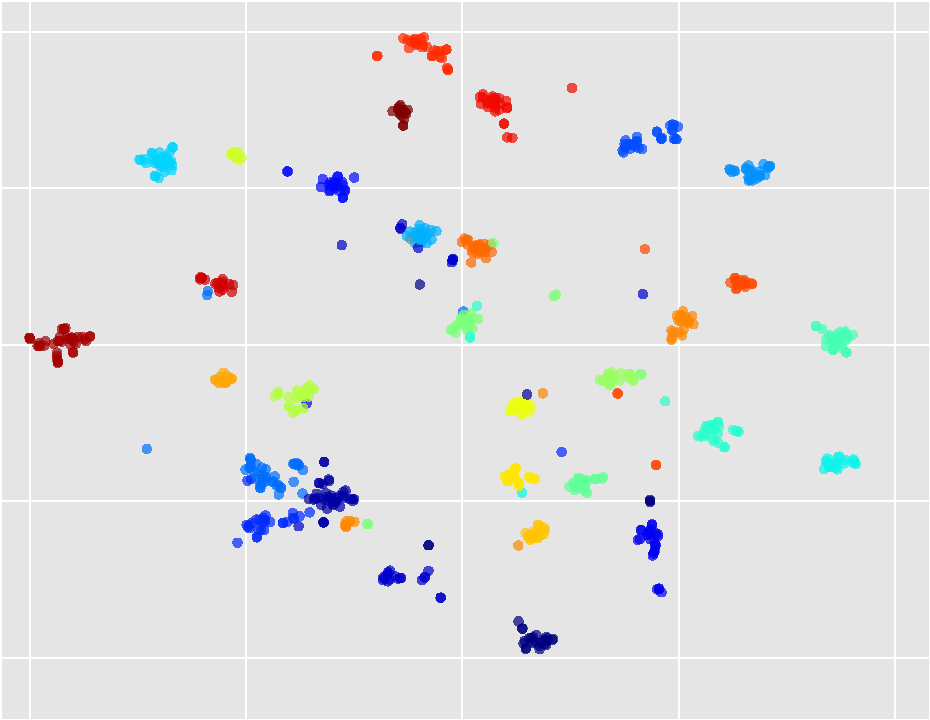
\includegraphics[width=\textwidth]{after_c_t_c}
        \caption{T with Adaptation}
    \end{subfigure}
    \caption{tSNE plots for office dataset Webcam(S)$\rightarrow$Amazon(T). Source features were discriminative and stayed discriminative as expected. On the other hand, target features became quite discriminative after the adaptation.}
    \label{fig:tsne}
        \includegraphics[width=\textwidth]{out_im.png}
        \vspace{-5mm}
\caption{tSNE plot for SVHN$\rightarrow$MNIST experiment. Please note that the discriminative behavior only emerges in the unsupervised target instead of the source domain. This explains the motivation behind modeling the problem as transduction. In other words, our algorithm is designed to be accurate and discriminative in the target domain which is the domain we are interested in.  }
\label{fig:tsnedigit}
\end{figure*}

\section{Conclusion} 
We described a transductive approach to the unsupervised domain adaptation problem by defining a joint learning problem on the transductive target label assignment and a asymmetric similarity metric across the domains. We further described a method to learn deep features which are discriminative in the target domain. Experimental results on digit classification using MNIST\cite{mnist} and SVHN\cite{svhn} as well as on object recognition using Office\cite{office} dataset show state of the art performance with a significant margin. We will make our learned models as well as the source code available immediately upon acceptance.



\clearpage
\bibliography{domain_transduction}
\bibliographystyle{icml2016}

\end{document} 